%!TEX root=paper.tex

% \newpage
\subsection{Web Article Reader}

The Web Article Reader allows the learners to subscribe to various sources of articles (e.g. websites, blogs) and provides a convenient interaction for reading and translating unknown words. 

% It consists of several components:

\subsubsection{Subscribing to Sources}
% \ml{make sure that we use source consistently in the text; not feed for example.}
From the user's point of view, the Reader is organized around {\em sources\xspace} of articles. The system categorizes sources by their language. Figure \ref{fig:system_subscriptions} presents the source subscription dialog, which in figure is displaying multiple sources for French. 


    \begin{figure}[h!]
    \centering
      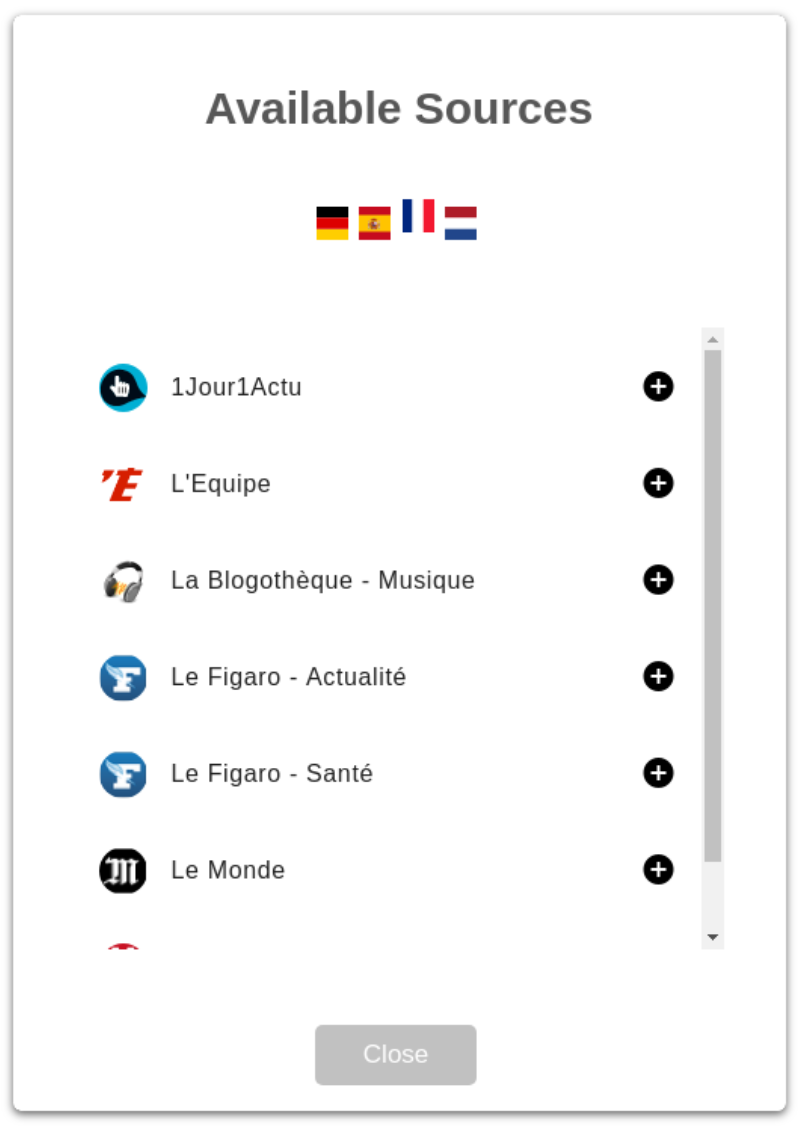
\includegraphics[width=0.4\columnwidth]{figures/available_sources}
      \caption{Different users subscribe to different sources}~\label{fig:system_subscriptions}
    \end{figure}

At the moment, multiple sources for every language are pre-loaded in the system and if a reader wants to add a new source they have to send an email to the maintainers of the system. 

A multi-lingual learner can subscribe to multiple sources in different languages. Once a reader is subscribed to a source, that source is constantly monitored and when new articles are detected, they are recommended to the learner. 

\subsubsection{Article Listing}

Article listing presents the source, a summary of the article, and an estimated difficulty level of the article.

    \begin{figure}[h!]
    \centering
      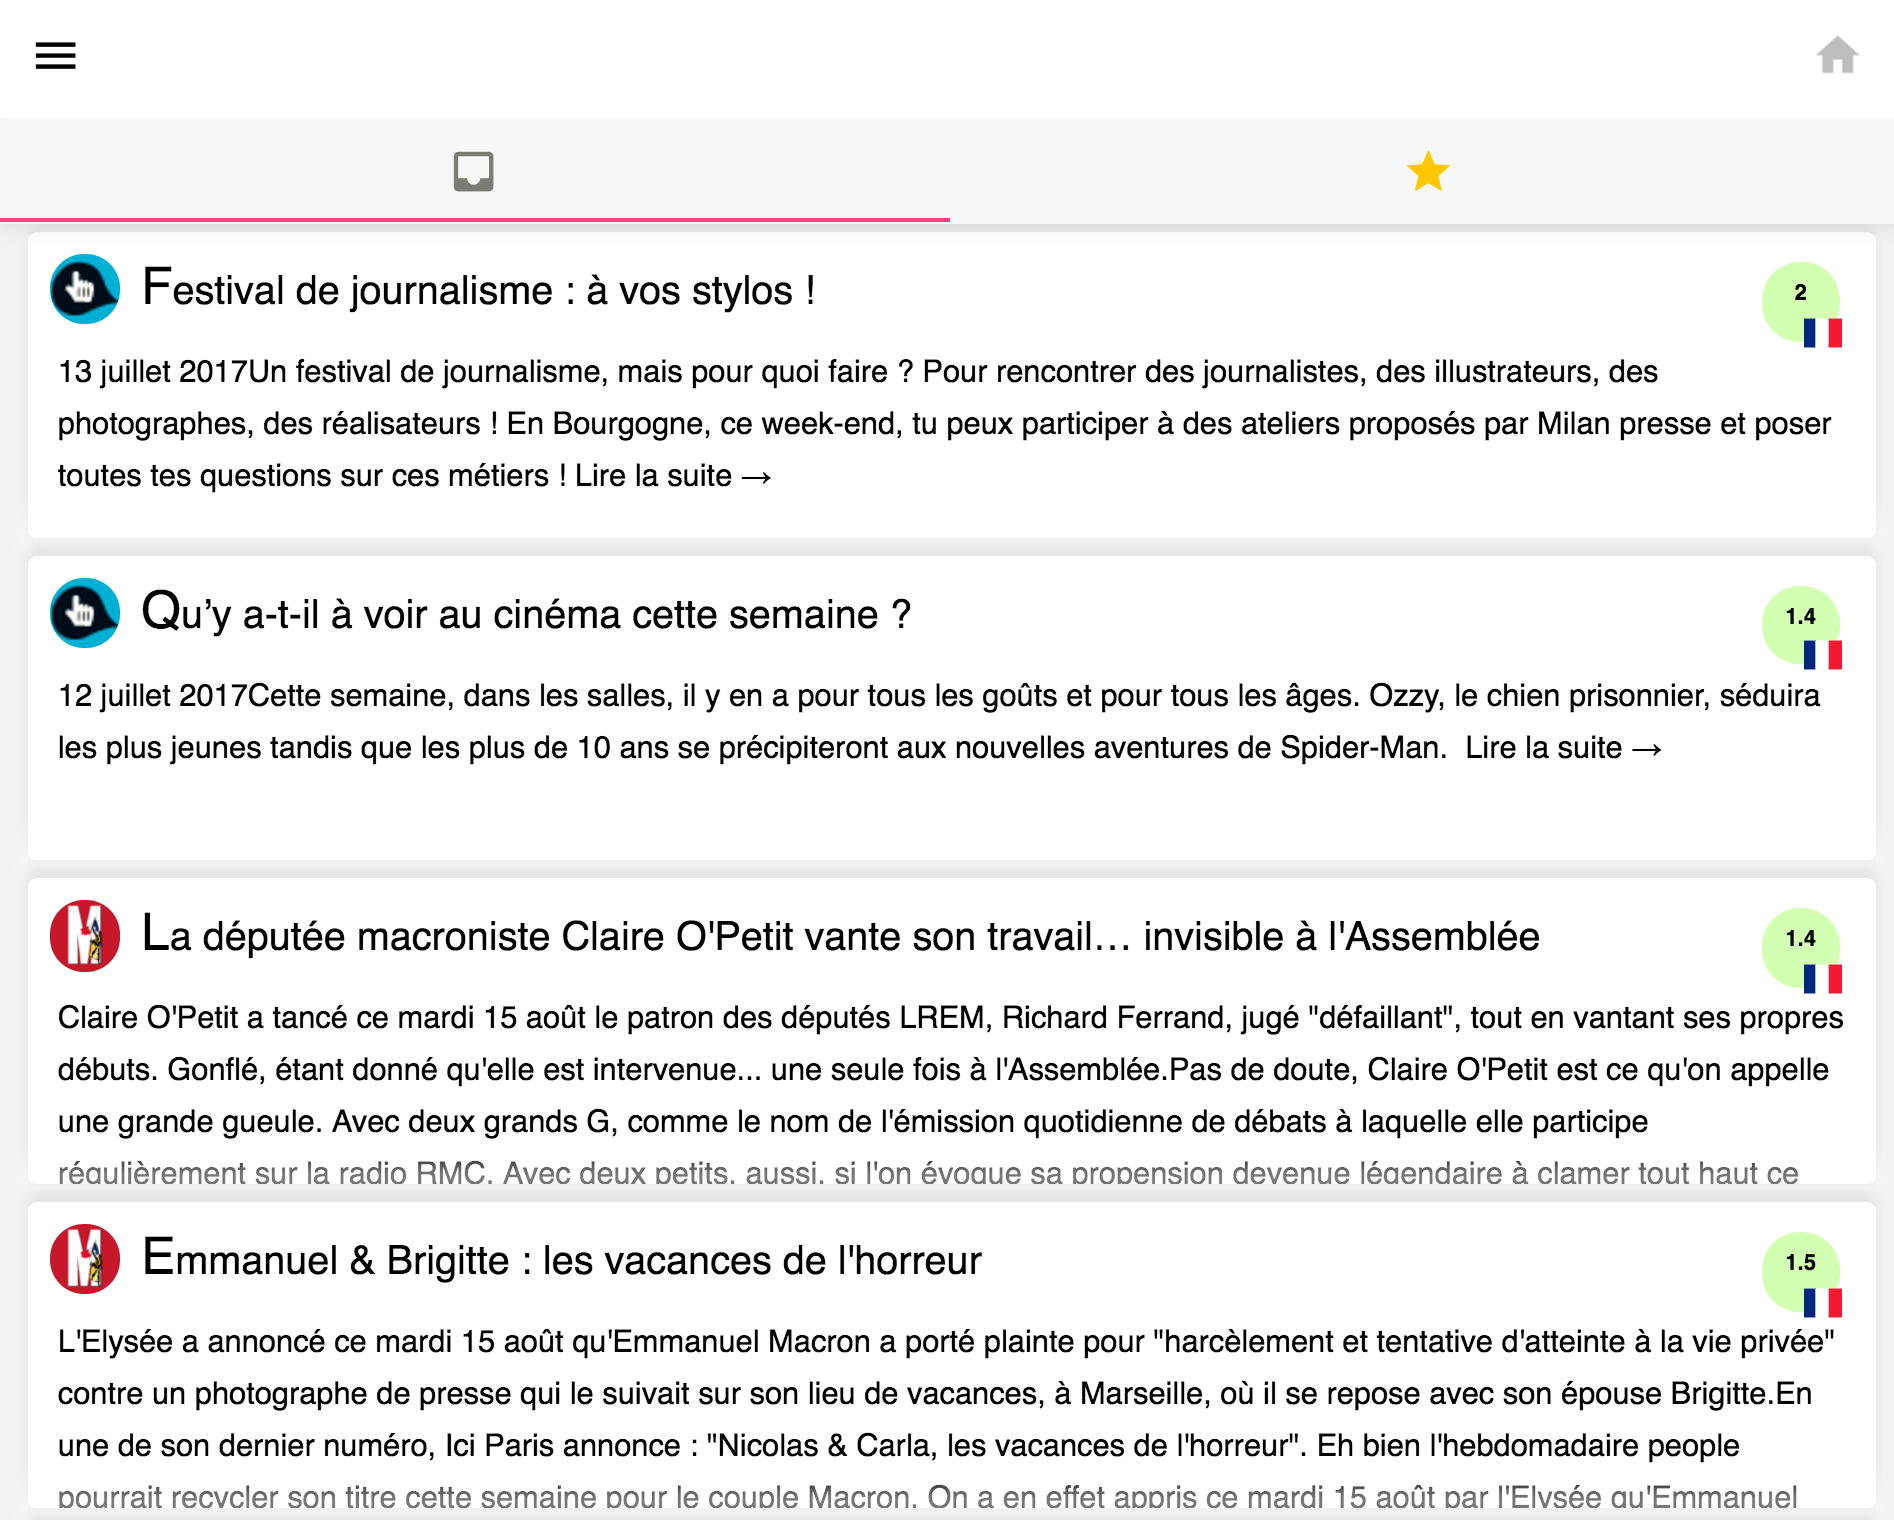
\includegraphics[width=0.75\columnwidth]{figures/article_listing}
      \caption{Article listing presents the source, a summary of the article, and an estimated difficulty level of the article }~
      \label{fig:registrations}
    \end{figure}


In order to properly visualize the reading difficulty of an article in an intuitive manner, there are three levels of information displayed here. First we display a flag representing the language of the article since a learner could be actually registered to feeds in multiple languages. Second, we allow the user to rapidly judge difficulty on an intuitive level by color coding the difficulty from green to yellow to red. When a particular article has grasped the user's attention, we allow for a more cognitive judgment by scoring the article from 0 to 5 in difficulty.

Difficulty estimation takes into account the frequency of the vocabulary items in the text. The system filters out articles that are too difficult given that it was deployed with non-advanced learners.\footnote{This is one of the limitations of the system that we discuss later.}

\subsubsection{Translations}

To make reading as facile as possible, the reader is optimized for the most frequent action that a reader is likely to want to perform: translating a word. Thus, when a user clicks on a word, a translation is inserted right after the word, as Figure \ref{fig:translated_word} illustrates: 

\begin{figure}[h!]
\centering
  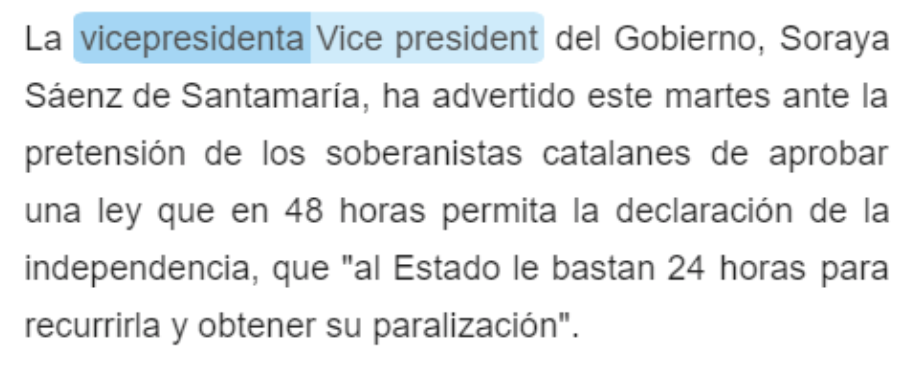
\includegraphics[width=0.8\columnwidth]{figures/translated_word}
  \caption{A translated word is inserted after the tapped word.}~\label{fig:translated_word}
\end{figure}

Other alternatives that we explored and eventually dropped (for each had disadvantages) were: 
\begin{description}

  \item [Temporarily showing a popup of the translation] and then hiding it again. This had a disadvantage for difficult sentences, where multiple words must be translated. The reader can forget translated words by the time they arrive at the end of an article, requiring them to re-translate.
  \item [Using the native selection mechanism] to select text as opposed to click / touch. 
  % We experimented with allowing the learner to select a word in the same way this is normally done on the corresponding platform. 
  This had the disadvantage that native selection is not designed as a priority action and thus is slow to respond (e.g. on Android a user must hold their fingertip down for almost a second before the contextual menu is displayed). 
\end{description}


\subsubsection{Chaining Translations}

The user can chain a few consecutive words into a single translation by simply tapping adjacent words which are then automatically merged in a translation bubble (Figure \ref{fig:translation_extension}). This is useful for collocations and in cases where by expanding the translated set of words the precision of the translation increases. 

    \begin{figure}[h!]
    \centering
      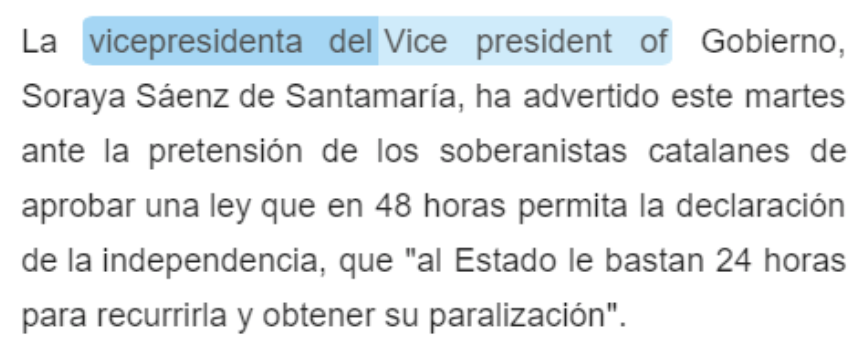
\includegraphics[width=0.8\columnwidth]{figures/translated_words1}
      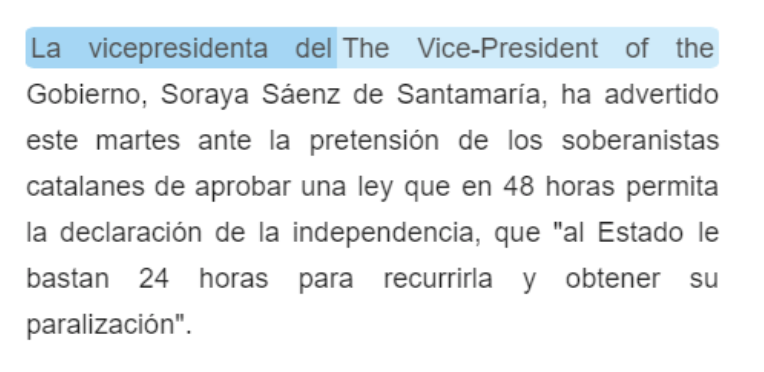
\includegraphics[width=0.8\columnwidth]{figures/translated_words2}
      \caption{When adjacent words are tapped the translation bubble is extended accordingly}~\label{fig:translation_extension}
    \end{figure}

This minimalistic interaction model serves a double purpose - it enables and eases the translation of several chained words but it discourages users from translating entire sentences or phrases. This is good because it is in line with the recommendations of the literature (e.g. Renandya argues that extensive reading should discourage intensive use of translations\cite{renadya07-power}) but also because it reduces the amount of characters which are being translated by the learner (and thus the costs of the system, since some of the translation services have a per-character fee). 

One of the limitations of this interaction is that it is not clear (at least at the moment) how to expand it for the situations in which expressions are present that are composed of words which are not adjacent (e.g. particle verbs in German and Dutch).


\subsubsection{Alternate Translations}
Due to the limitations of machine translation multiple translations might be possible in a given context. In such a case the system will insert the most likely alternative as described earlier right after the selected text, but it will allow the reader to discover alternatives. With a click on the translation, a drop-down menu appears in which alternatives are presented. Figure \ref{fig:registrations} shows that besides the predefined alternatives the learner can provide their own translation via an input box (the third line, ``took place'' is typed in by the learner in the figure). 


\begin{figure}[h!]
\centering
  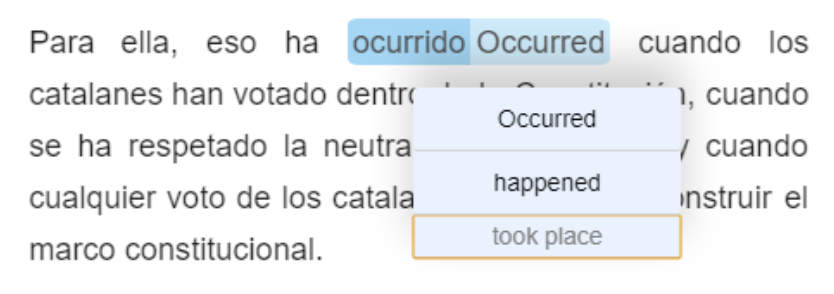
\includegraphics[width=0.8\columnwidth]{figures/translation_alter_menu}
  \caption{A translated word is inserted after the tapped word.}~\label{fig:registrations}
\end{figure}

\subsubsection{Pronounciation}

The process we followed while developing the reader was an iterative process, with short release cycles (one or two weeks), and frequent testing with members of the research team, and the occasional external user. 

One of the features that we added following a suggestion of an early beta-tester -- a teacher of Dutch as a foreign -- was the pronounciation of a translated word. After exploring several trade-offs between flexibility, ease of use, and a clean user interface, we settled on triggering the pronounciation of a word (or group of words in a selection bubble) with a tap on them. 

The pronounciation is generated by using the HTML5 Speech API which is supported by most modern browsers both on the mobile and on the desktop. 

% \ml{could ask the users if they are happy with it.}
% Although no user has yet complained about it, this means that a user can not pronounce a word without it being translated first. It might also be that for some languages this is more important than for others, and we just did not have users learning those languages (e.g. Danish is notoriously hard to pronounce). In the future we plan to expand the interaction modes to allow pronounciation to exist seperately from translation.